\documentclass[10pt]{article}
\usepackage[font={small}, justification=justified, singlelinecheck=false]{caption}
\usepackage{graphicx}

\begin{document}

Figure created using Inkscape Vector Graphics software.

\begin{figure}[!ht]
  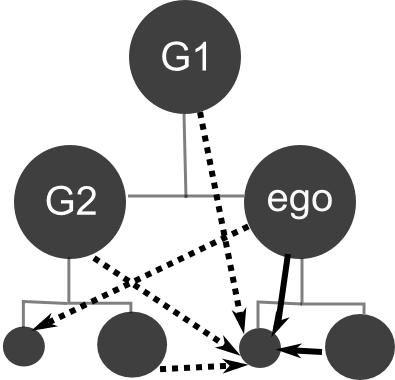
\includegraphics{Fig1.png}
\caption{Circles represent actors in the simulation and bars represent the kinship links between them.  The larger circles in the third generation represent care-giving offspring.  Solid lines show residence independent caring relationships, while dotted lines show caring relationships unique to the natal household.  Note, the number of offspring starts at 0 and grows throughout the simulation.}
\label{fig:kin_diag}       % Give a unique label

\end{figure} 

\end{document}
